\chapter{Experimental setup}
In this chapter we describe the setup we use for our experiments. All results of our experiments, as displayed in chapter \ref{ch:results}, are measured over a corpus of Java projects. In this chapter we will explain how we prepared this corpus.

\section{The corpus}\label{chap:corpus}
For our measurements we use a large corpus of open source projects \cite{githubCorpus2013}. This corpus has been assembled to contain relatively higher quality projects. Also, any duplicate projects were removed from this corpus. This results in a variety of Java projects that reflect the quality of average open source Java systems and are useful to perform measurements on.

As indicated in chapter \ref{chap:challenge} CloneRefactor requires all libraries of software projects we test. As these are not included in the used corpus \cite{githubCorpus2013}, we decided to filter the corpus to only include Maven projects. Maven is a build automation tool used primarily for Java, and works on basis of an \texttt{pom.xml} file to describe the projects' dependencies. As no \texttt{pom.xml} files are included in the corpus, we cloned the latest version of each project in the corpus. We then removed each project that has no \texttt{pom.xml} file. As a final step, we collected all dependencies for each project by using the \texttt{mvn dependency:copy-dependencies -DoutputDirectory=lib} Maven command, and removed each project for which not all dependencies were available (due to non-Maven dependencies being used or unsatisfiable dependencies being referenced in the \texttt{pom.xml} file).

Some general data regarding this corpus is displayed in Table \ref{table:general}.

\begin{table}[H]
  \begin{center}
  \caption{General results for GitHub Java projects corpus \cite{githubCorpus2013}.} \label{table:general}
  \medskip
\begin{tabular}{|l|l|}
\hline
Amount of projects                                                                                      & 1,361      \\ \hline
\begin{tabular}[c]{@{}l@{}}Amount of lines (excluding\\whitespace, comments and newlines.)\end{tabular} & 1,414,996  \\ \hline
Amount of statements/declarations                                                                       & 1,212,189  \\ \hline
\begin{tabular}[c]{@{}l@{}}Amount of tokens (excluding\\whitespace, comments and newlines.)\end{tabular} & 11,643,194 \\ \hline
\end{tabular}
\end{center}
\end{table}

\section{Context Analysis of Clones}\label{chap:contextsetup}
To be able to refactor code clones, it is important to consider the context of the clone. We define the following aspects of the clone as its context:
\begin{enumerate}
  \item \textbf{Relation:} The relation of clone instances among each other through inheritance.
  \item \textbf{Location:} Where a clone instance occurs in the code.
  \item \textbf{Contents:} The statements/declarations of a clone instance.
\end{enumerate}
We perform experiments on each of these aspects, defining categories and measuring these categories over the corpus.

\begin{figure}[H]
    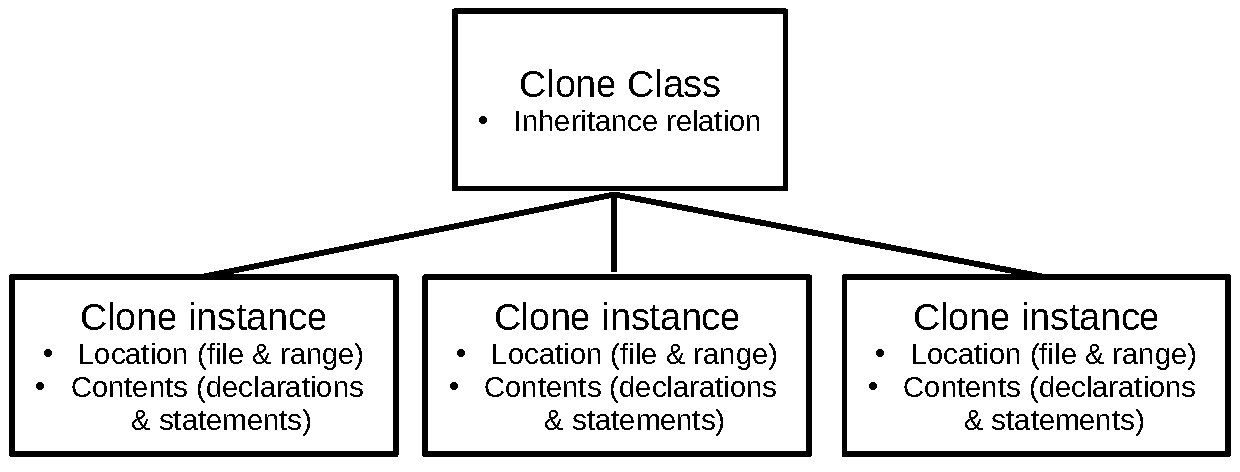
\includegraphics[width=0.6\columnwidth]{img/context}
    \caption{Abstract representation of clone classes and clone instances.}
  \label{fig:clonecontext}
\end{figure}

Fig.~\ref{fig:clonecontext} shows an abstract representation of clone classes and clone instances. The relation of clones through inheritance is measured for each clone class. The location and contents of clones are measured for each clone instance.

\subsection{Relation}\label{sec:setuprelation}
When merging code clones in object-oriented languages, it is important to consider the inheritance relation between clone instances. This relation has a big impact on how a clone should be refactored.

Fontana et al.~\cite{fontana2015duplicated} describe measurements on 50 open source projects on the relation of clone instances to each other. To do this, they first define several categories for the relation between clone instances in object-oriented languages. These categories are as follows:
\begin{enumerate}
  \item \textbf{Same Method}: All instances of the clone class are in the same method.
  \item \textbf{Same Class}: All instances of the clone class are in the same class.
  \item \textbf{Superclass}: All instances of the clone class are in a class that is child or parent of each other.
  \item \textbf{Ancestor Class}: All instances of the clone class are superclasses except for the direct superclass.
  \item \textbf{Sibling Class}: All instances of the clone class have the same parent class.
  \item \textbf{First Cousin Class}: All instances of the clone class have the same grandparent class.
\item \textbf{Same Hierarchy Class}: All instances of the clone class belong to the same inheritance hierarchy, but do not belong to any of the other categories.
\item \textbf{Same External Superclass}: All instances of the clone class have the same superclass, but this superclass is not included in the project but part of a library.
\item \textbf{Unrelated class}: There is at least one instance in the clone class that is not in the same hierarchy.
\end{enumerate}

We added the following categories, to gain more information about clones and reduce the number of unrelated clones:

\begin{enumerate}
\item \textbf{Same Interface}: All instances of the clone class are in a class or interface that have a common interface anywhere in their inheritance hierarchy.
\item \textbf{No Direct Superclass}: All instances of the clone class are in a class that does not have any superclass.
\item \textbf{No Indirect Superclass}: All instances of the clone class are in a class that does not have any external classes in its inheritance hierarchy.
\end{enumerate}

Figure \ref{fig:clonecontext} shows an abstract representation of clone classes and clone instances. The relation of clones through inheritance is measured on clone class level: it involves all child clone instances. The location and contents of clones is measured on clone instance level. A clone's location involves the file it resides in and the range it spans (for example: line 6 col 2 - line 7 col 50). A clone instance contents consists of a list of all statements and declarations it spans.

\begin{figure}[H]
  \caption{Abstract figure displaying relations of clone classes. Arrows represent superclass relations.}
    \medskip
    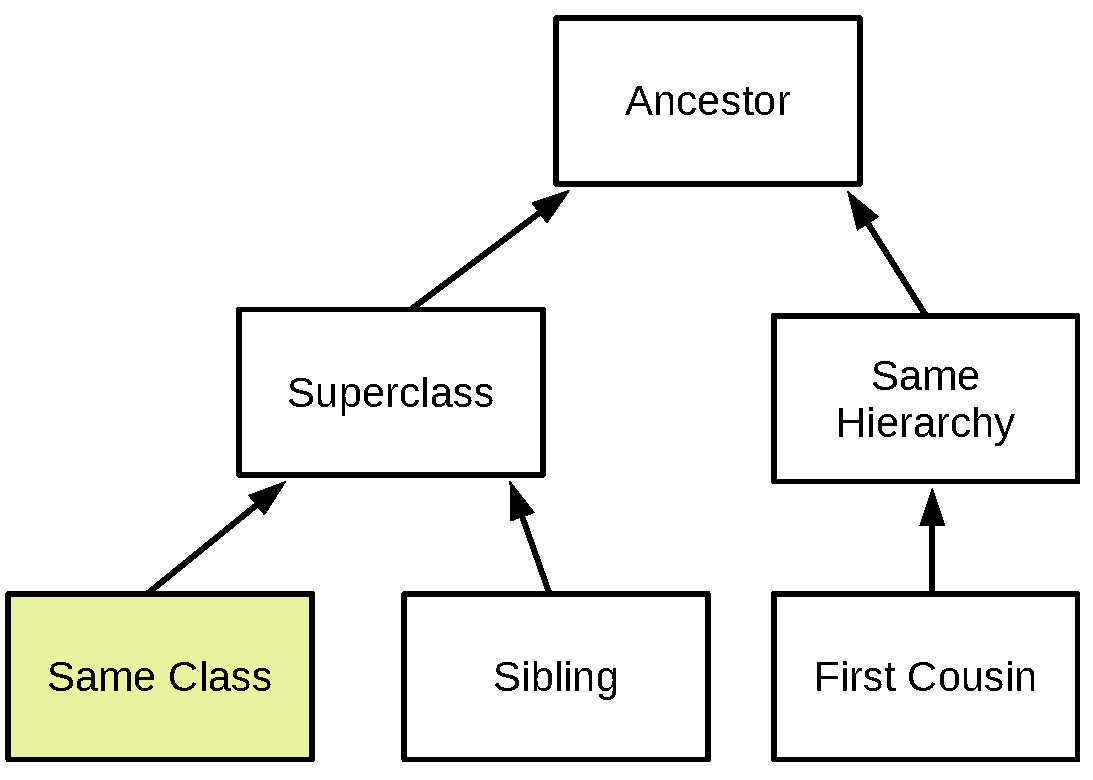
\includegraphics[width=1\columnwidth]{img/Relation}
  \label{fig:clonerelation}
\end{figure}

We separate these relations into the following categories, because of their related refactoring opportunities:
\begin{itemize}
  \item \textbf{Common Class}: \textit{Same Method}, \textit{Same Class}
  \item \textbf{Common Hierarchy}: \textit{Superclass}, \textit{Ancestor Class}, \textit{Sibling Class}, \textit{First Cousin}, \textit{Same Hierarchy}
  \item \textbf{Common Interface}: \textit{Same Interface}
  \item \textbf{Effectively Unrelated}: \textit{No Direct Superclass}, \textit{No Indirect Superclass}, \textit{External Superclass}, \textit{Unrelated}
\end{itemize}

Every clone class only has a single relation, which is the first relation from above list that the clone class applies to. For instance: all ``Superclass'' clones also apply to ``Same Hierarchy'', but because ``Superclass'' is earlier in above list they will get the ``Superclass'' relation. This is because the items earlier in the list denote a more favorable refactoring.

\subsubsection{Common Class}
The \textit{``Same method''} and \textit{``Same class''} relations share a common refactoring opportunity. Clones of both these catagories, when extracted to a new method, can be placed in the same class. Both of these relations are most favorable for refactoring, as they require a minimal design tradeoff. Furthermore, global variables that are used in the class can be used without having to create method parameters.

A clone class is flagged as ``Same method'' if all clone instances in the clone class are in the same method:

\begin{equation}\label{eq:samemethod}
\forall (i_1 \in C) \forall (i_2 in C) Mi_1 = Mi_2
\end{equation}

Where \textit{M} is the method in which a clone instance is found. Please note that a clone instance may not always be in a method, for which this predicate will fail. Each node in a clone instance is checked for this predicate, so if a single node of a clone instance is outside a method, the predicate will fail.

A clone class is flagged as ``Same class'' if all clone instances in the clone class are in the same class:

\begin{equation}\label{eq:samemethod}
\forall (i_1 \in C) \forall (i_2 in C) Di_1 = Di_2
\end{equation}

Where \textit{D} is the class declaration in which the clone instance is found.

\subsubsection{Common Hierarchy}
Clones that are in a common hierarchy can be refactored by using the ``Extract Method'' refactoring method followed by ``Pull Up Method'' until the method reaches a location that is accessible by all clone instances. However, the more often ``Pull Up Method'' has to be used, the more detrimental the effect is on system design. This is because putting a lot of functionality in classes higher up in an inheritance structure can result in the ``God Object'' anti-pattern. A god object is an object that knows too much or does too much.



\subsubsection{Common Interface}
\todo{TODO}

\subsubsection{Effectively Unrelated}
\todo{TODO}

\subsection{Location}\label{sec:setuplocation}
A paper by Lozano et al. \cite{lozano2007evaluating} discusses the harmfulness of cloning. The authors argue that 98\% are produced at method-level. However, this claim is based on a small dataset and based on human copy-paste behavior rather than static code analysis. We validated this claim over our corpus. The results for the clone instance locations are shown in Table \ref{table:locations}. We chose the following categories:
\begin{enumerate}
  \item \textbf{Method/Constructor Level:} A clone instance that does not exceed the boundaries of a single method or constructor (optionally including the declaration of the method or constructor itself).
  \item \textbf{Class Level:} A clone instance in a class, that exceeds the boundaries of a single method or contains something else in the class (like field declarations, other methods, etc.).
  \item \textbf{Interface Level:} A clone that is (a part of) an interface.
  \item \textbf{Enumeration Level:} A clone that is (a part of) an enumeration.
\end{enumerate}

\subsection{Contents}\label{sec:setupcontents}
Finally, we looked at what nodes individual clone instances span. We selected the following categories to be relevant for refactoring:
\begin{enumerate}
  \item \textbf{Full Method/Class/Interface/Enumeration:} A clone that spans a full class, method, constructor, interface or enumeration, including its declaration.
  \item \textbf{Partial Method/Constructor:} A clone that spans a method partially, optionally including its declaration.
  \item \textbf{Several Methods:} A clone that spans over two or more methods, either fully or partially, but does not span anything but methods (so not fields or anything in between).
  \item \textbf{Only Fields:} A clone that spans only global variables.
  \item \textbf{Includes Fields/Constructor:} A clone that spans a combination of fields and other things, like methods.
  \item \textbf{Method/Class/Interface/Enumeration Declaration:} A clone that contains the declaration (usually the first line) of a class, method, interface or enumeration.
  \item \textbf{Other:} Anything that does not match with above-stated categories.
\end{enumerate}

\section{Method extraction opportunities}\label{sec:refactorabilitysetup}
The most used technique to refactor clones is method extraction (creating a new method on basis of the contents of clones). However, method extraction cannot be applied in all cases. In these instances, more conditions may apply to be able to conduct a refactoring, if beneficial at all.

We measured the number of clones that can be refactored through method extraction (without additional transformations being required). We defined the following categories:
\begin{itemize}
    \item \textbf{Can be extracted:} This clone is a fragment of code that can directly be extracted to a method. Then, based on the relation between the clone instances, further refactoring techniques can be used to refactor the extracted methods (for instance ``pull up method'' for clones in sibling classes).
    \item \textbf{Complex control flow:} This clone contains \texttt{break}, \texttt{continue} or \texttt{return} statements, obstructing the possibility of method extraction.
    \item \textbf{Spans part of a block:} This clone spans a part of a statement.
    \item \textbf{Is not a partial method:} If the clone does not fall in the ``Partial method'' category of Table~\ref{table:contents}, the ``extract method'' refactoring technique cannot be applied.
\end{itemize}
